\section{Integrated rejector}~\label{sec:integrated_rejector}

The integrated rejector combines the rejector and predictor into a single model where it is impossible to distinguish between the role of the $h$ and the $r$.  
Formally, the model with integrated reject option acts as
\begin{equation}
    m(x) \in \mathcal{Y} \cup \{\rr{}\}.
	\label{eq:integrated_rejector}
\end{equation}
Conceptually, this model simply includes $\rr{}$ as an additional output.

This architecture usually needs a unique algorithm for learning predictor  and rejector in tandem~\citep{Cortes2016,Cortes2016b}. 
There are two distinct approaches to learning an integrated rejector. The first approach is model-agnostic and involves designing an objective function that penalizes (mis)predictions as well as rejections. The second approach is model-specific and entails integrating a rejector into an existing predictor, where rejection becomes part of the decision-making process.

\paragraph{\bf{Learning a model-agnostic integrated rejector.}}
Typically, learning a model that simultaneously makes accurate predictions and rejects the examples that will be otherwise mispredicted can be done by simply designing a specialized objective function~\citep{Mozannar2020}. Then, such a function can be minimized using potentially any existing optimizer, which makes it model-agnostic.
\changed{For instance, for classification, a simple cost-based objective for any hypothesis $m$ can be expressed as
% \begin{equation*}
%     L = \E_{p(X,Y)} \left[C_c \mathbbm{1}_{m(x) = y}(x) + C_r \mathbbm{1}_{m(x) = \rr{}}(x) + C_e \mathbbm{1}_{m(x) \not\in \{y,\rr{}\}}(x)\right].
% \end{equation*}
\begin{equation*}
    L = \E_{p(X,Y)} \left[C_r \mathbbm{1}_{m(x) = \rr{}}(x) + \mathbbm{1}_{m(x) \not\in \{y,\rr{}\}}(x)\right]
\end{equation*}
with $C_r \in (0, 1/2]$.
}
For tasks other than classification, ad-hoc loss functions are used, such as those for multilabel classification~\citep{Pillai2013,Nguyen2020,Nguyen2021}, regression~\citep{Asif2020,Kalai2021}, online learning~\citep{pmlr-v80-cortes18a,Kocak2020}, and multi-instance learning~\citep{Zhang2006}. However, in many cases, surrogate losses are employed to enable efficient optimization, as learning from discrete losses is computationally impractical~\citep{Wegkamp2007,Grandvalet2009,Cao2022}. Consequently, the original loss $L$ is converted into a convex loss by utilizing surrogate functions $\psi \colon \mathbb{R} \to \mathbb{R}$, such as the logistic and hinge functions~\citep{Ramaswamy2018,Zhang2018,Bartlett2008}:
\begin{equation*}
    \text{Logistic: } \psi(L) = \frac{1}{1+ \exp(L)}, \qquad \text{Hinge: } \psi(L) =
    \begin{cases}
        1- \frac{1-C_r}{C_r} L & \text{ if } L<0\\
        1-L  & \text{ if } 0 \le L < 1\\
        0 & \text{ otherwise}
    \end{cases}
\end{equation*}
\changed{For the hinge loss to be convex, it is required that $C_r \leq 1/2$ which is the case for classification as otherwise the cost of rejection would be higher than the cost of random guessing.}
Numerous studies in the literature have explored the properties of surrogate loss functions~\citep{Yuan2010}, including calibration effects~\citep{Ni2019,Charoenphakdee2019}, estimates of bounds for misclassification risk~\citep{Shekhar2019,Kato2020}, penalization effects in high-dimensional spaces~\citep{Wegkamp2012}, proximity to the optimal Bayes solution~\citep{Bounsiar2008,Shen2020}, and convergence rate analysis~\citep{Denis2020}.

Lastly, one can allocate an extra class $K+1$ (commonly known as the \emph{reject class}) for rejection and assign a specific penalization cost $C_r$ for predicting such a class. With this setting, there are two main alternatives. In the first case, there are no actual examples belonging to this class. Thus, these approaches design loss functions to enable the classifier to assign on its own a positive score to ambiguous examples~\citep{Huang2020,Feng2022}. For instance, \citet{Ziyin2019} \changed{propose to measure the expected loss as}
\begin{equation*}
L = \mathbb{E}_{p(X,Y)} \left[\log(s_{k}(x) + \frac{1}{C_r} s_{K+1}(x))\right],
\end{equation*}
where $s_{k}(x)$ and $s_{K+1}(x)$ are probabilities, respectively, for the class $y = k$ and $K+1$ (rejection). At a high level, decreasing the rejection cost $C_r$ results in higher chances of rejection. In the second case, one artificially generates examples ${x_{n+1},\dots,x_{N}}$ (e.g., adversarial examples) and assigns them to the rejection class $K+1$. By training a predictor with $K+1$ classes, the reject option is naturally incorporated as output, and any (multi-class) predictor can be used for novelty~\citep{Vasconcelos1995,Singh2004,Urahama1995} or ambiguity rejection~\citep{Thulasidasan2019,Pang2022}.


\paragraph{\bf{Learning a model-specific integrated rejector.}}

\begin{figure}
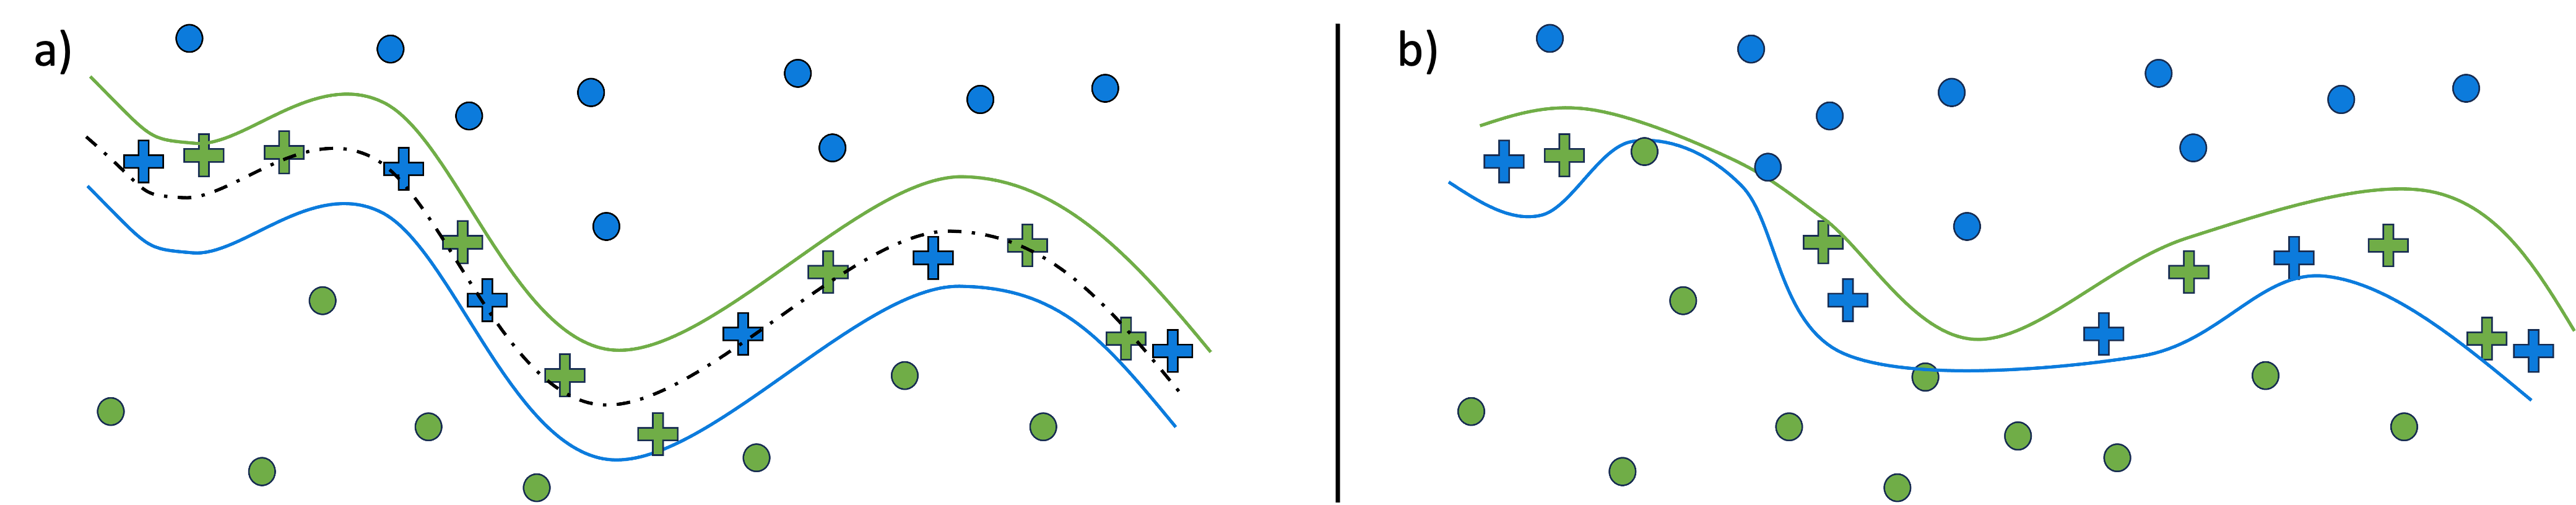
\includegraphics[width=\linewidth]{svms.png}
\caption{Two cases of Integrated SVMs: (a) on the left side, the two hyperplanes are parallel and equidistant to the decision boundary (dashed line); (b) on the right side, each SVM gives higher priority to one class by limiting mispredictions.}
\label{fig:integrated_svm}
\end{figure}

In many practical use cases, one may already know that a specific class of models works well within the given context, such as SVM models in medical applications~\citep{Hanczar2008,Hamid2017}. Given a specific predictor, its learning algorithm can be slightly adapted to include the reject option. 
For instance, \emph{integrated SVMs} set two (or more) hyperplanes on the feature space and reject all the examples located in between them~\citep{Pillai2011,Lin2018,Zidelmal2012HeartbeatCU}. 
Figure~\ref{fig:integrated_svm} shows two common cases to learn the hyperplanes. First, one can parametrize the hyperplane as $w\cdot x + b \pm \varepsilon = 0$, with $\varepsilon\ge 0$, which results in parallel and equidistant hyperplanes from the decision boundary, where $\varepsilon$ indicates the distance~\citep{Fumera2002}. Learning such hyperplanes requires minimizing the empirical loss
\begin{equation*}
    L = \frac{1}{2} w \cdot w + C \sum_{i=1}^n l(\xi_i, \varepsilon) - \sum_{i=1}^n \alpha_i\left[y_i(w\cdot x_i+b)-1+\xi_i\right]
\end{equation*}
where $w$ is the weight vector, $b$ is the intercept of the hyperplane, $C$ is a (large) hyperparameter that regulates the importance of the performance/rejection trade-off expressed inside the function $l(\xi_i,\varepsilon)$, and $\alpha_i$ are the Lagrangian multipliers. Second, the two hyperplanes can be parametrized as 
\begin{equation*}
    w'\cdot x + b' = 0 \quad \text{and} \quad w''\cdot x + b'' = 0.
\end{equation*}
By formulating two distinct optimization problems, one can learn the parameters of these hyperplanes. In this approach, one hyperplane is highly penalized for mispredicting the positive class, while the other one is for the negative class. Essentially, this technique yields two SVMs that have few mispredictions on either class, and examples falling in between the hyperplanes can be naturally rejected~\citep{Varshney2006}.
With the same approach, one can also learn a \gls{ocsvm} for each class to reject test examples that lie outside any learned hypersphere (novelty) or within two overlapping hyperspheres (ambiguity)~\citep{Lotte2008,Loeffel2015,Wu2007}. Finally, \citet{Sousa2014a} shows that limiting the number of support vectors reduces the computational cost, while still ensuring high performance in most cases.

However, in several cases, more than two SVMs are used. For instance, in multi-label classification one can exploit as many SVMs as the number of labels and fit each hyperplane to discriminate between one class and all the others~\citep{Pillai2011}. This raises the issue of defining rejection in the regions of intersection between some, but not all, of the hyperplanes. To address this, a natural solution is to utilize a data-replication method~\citep{Sousa2009b}. This approach involves replicating the complete dataset for each class $k \in \mathcal{Y}$, adding a new dimension $z$ with the class number, changing the target variable of each replica to a discrete one-vs-all label, and discriminating class $k$ from the other classes~\citep{Cardoso2007,DaRochaNeto2011}.

Finally, \emph{Neural Network models}  allow integrating the rejector and predictor into the same structure by modifying their output layers~\citep{Gangrade2021,Ziyin2019}.  \citet{Geifman2019b} propose to introduce an additional head $m_r$ into the network that is dedicated to rejection. Specifically, $m_r$ is set as a sigmoid function and used such that 
\begin{equation*}
    m(x) = \rr{} \quad \text{ if } m_r(x) < 0.5.
\end{equation*}
Similar to the SVM case, \citet{GascaA.2011} and \citet{Mesquita2016} measure the disagreement of two Neural Networks trained to prioritize the classes differently. Specifically, they assume a binary classification task and use the output of two neural networks $h_1$, $h_2$ to predict the positive class if $h_1(x), h_2(x) \ge 0$, the negative class if $h_1(x), h_2(x) < 0$ and rejection if they disagree on the sign. For this task, they use two weighted Extreme Learning Machines (wELM)~\citep{Zong2013}, namely two neural networks with $Q$ hidden neurons that output 
$$h_*(x) = \sum_{q=1}^Q w_y \beta_q g(a_q \cdot x + b_q)$$
where $w_y$ is the cost related to the example $x$ that belongs to the class $y$, $a_q$ is the weight vector connecting the $q$-th hidden node and the input nodes, $b_q$ is the bias of the $q$-th hidden node and $g$ is the activation function. By setting the class misprediction costs, learning the parameters $\beta = (\beta_1,\dots,\beta_Q)$ requires using the traditional weighted least square formulation $\min \| H \beta - Y\|^2$ so that
\begin{equation*}
    \beta = (H^TWH)^{-1}H^TWY
\end{equation*}
where $H$ is the $n\times Q$ matrix of activation functions $h_{iq} = g(a_q \cdot x_i + b_q)$, $W$ is the $n\times 1$ matrix of class costs (one per example) and $Y$ is the target vector. Thus, each network limits one class mispredictions and the region of disagreement is designed to be the rejection region.

\paragraph{\bf{Benefits and drawbacks of an integrated rejector.}}
This architecture has two key \emph{benefits}.
First, integrating the predictor and rejector means that both aspects of the model are optimized toward the task at hand. 
This can improve the performance of the model with rejection when compared to using other architectures because the predictor's and the rejector's components can affect each other.
Second, because it is a unique model, the bias introduced by the model with rejection is potentially less than in the scenario where the predictor and rejector are two different models. 
However, this architecture has potential \emph{drawbacks}, as designing such a rejector might not be trivial. First, it requires extensive knowledge about the predictor in order to integrate the reject option. Second, it may require developing a novel algorithm to learn the model with a reject option from data. Finally, it is computationally more expensive than the other architectures, as any changes to the rejector require retraining the entire model, which can be time-consuming~\citep{Clertant2020,Shpakova2021}.
